% RQ1 at a glance --- simple high-level flow chart.
% Compile standalone:  pdflatex simple_flow_rq1.tex
% Or drop the tikzpicture into your thesis (needs \usepackage{tikz} + the listed libraries).
\documentclass[border=10pt]{standalone}
\usepackage{tikz}
\usetikzlibrary{arrows.meta, positioning, shapes.geometric}

\begin{document}
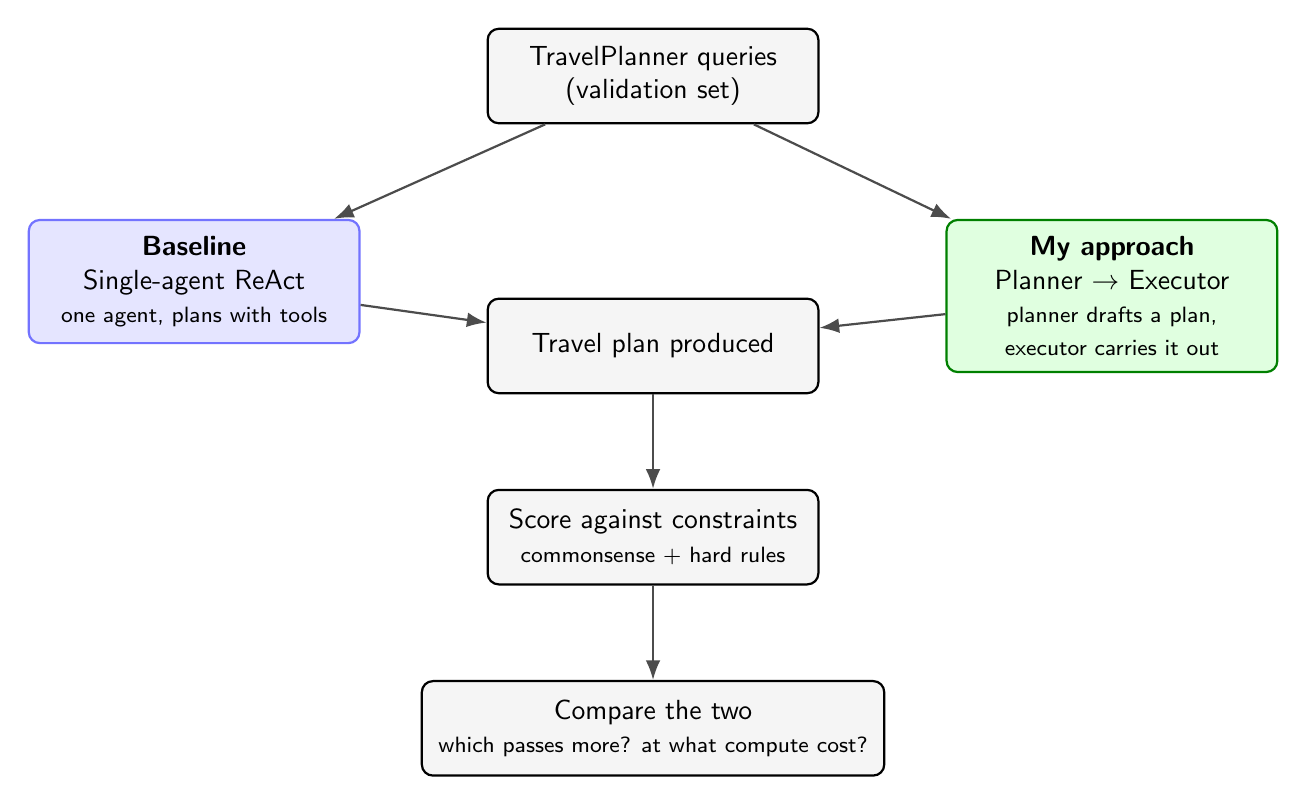
\begin{tikzpicture}[
    node distance = 12mm and 16mm,
    every node/.style = {font=\sffamily},
    box/.style = {rectangle, rounded corners=4pt, draw, thick,
                  align=center, minimum width=42mm, minimum height=12mm,
                  inner sep=6pt},
    neutral/.style = {box, fill=gray!8},
    base/.style    = {box, fill=blue!10, draw=blue!55},
    mine/.style    = {box, fill=green!12, draw=green!50!black},
    arr/.style     = {-{Latex[length=2.5mm]}, thick, gray!60!black}
  ]

  % nodes
  \node[neutral] (q) {TravelPlanner queries\\(validation set)};

  \node[base]  (b) [below left=of q]  {\textbf{Baseline}\\Single-agent ReAct\\\footnotesize one agent, plans with tools};
  \node[mine]  (p) [below right=of q] {\textbf{My approach}\\Planner $\rightarrow$ Executor\\\footnotesize planner drafts a plan,\\\footnotesize executor carries it out};

  \node[neutral] (r) [below=22mm of q] {Travel plan produced};
  \node[neutral] (e) [below=of r] {Score against constraints\\\footnotesize commonsense + hard rules};
  \node[neutral] (c) [below=of e] {Compare the two\\\footnotesize which passes more? at what compute cost?};

  % edges
  \draw[arr] (q) -- (b);
  \draw[arr] (q) -- (p);
  \draw[arr] (b) -- (r);
  \draw[arr] (p) -- (r);
  \draw[arr] (r) -- (e);
  \draw[arr] (e) -- (c);

\end{tikzpicture}
\end{document}
